\documentclass[12pt, twoside]{article}
\usepackage[letterpaper, margin=1in, headsep=0.2in]{geometry}
\setlength{\headheight}{0.6in}
%\usepackage[english]{babel}
\usepackage[utf8]{inputenc}
\usepackage{microtype}
\usepackage{amsmath}
\usepackage{amssymb}
%\usepackage{amsfonts}
\usepackage{siunitx} %units in math. eg 20\milli\meter
\usepackage{yhmath} % for arcs, overparenth command
\usepackage{tikz} %graphics
\usetikzlibrary{quotes, angles}
\usepackage{graphicx} %consider setting \graphicspath{{images/}}
\usepackage{parskip} %no paragraph indent
\usepackage{enumitem}
\usepackage{multicol}
\usepackage{venndiagram}

\usepackage{fancyhdr}
\pagestyle{fancy}
\fancyhf{}
\renewcommand{\headrulewidth}{0pt} % disable the underline of the header
\raggedbottom
\hfuzz=2mm %suppresses overfull box warnings

\usepackage{hyperref}

\fancyhead[LE]{\thepage}
\fancyhead[RO]{\thepage \\ Name: \hspace{4cm} \,\\}
\fancyhead[LO]{BECA / Dr. Huson / Geometry\\*  Unit 5: Pythagorean theorem \\* 6 December 2022}

\begin{document}

\subsubsection*{5.7 Final exam: Create equations to solve problems \hfill HSA.CED.A1}
\begin{enumerate}
\item Find $GH$, given $G=0.4$ and $H=5.6$.
\begin{flushright}
  \begin{tikzpicture}
    \draw[<->] (-1.5,0)--(7.5,0);
    \foreach \x in {-1,...,7}
      \draw[shift={(\x,0)},color=black] (0pt,-3pt) -- (0pt,3pt) node[below=5pt]  {$\x$};
      \draw[fill] (0.4,0) circle [radius=0.05] node[above] {$G$};
      \draw[fill] (5.6,0) circle [radius=0.05] node[above] {$H$};
  \end{tikzpicture}
\end{flushright} \vspace{2cm}

\item Given $\overline{ABC}$, $AB=2 \frac{1}{2}$, and $BC=5 \frac{3}{4}$. Find ${AC}$. \par \vspace{1cm}
  \begin{tikzpicture}
    \draw[thick] (0,0)--(8,0);
    \draw[fill] (0,0) circle [radius=0.05] node[below]{$A$};
    \draw[fill] (2.5,0) circle [radius=0.05] node[below]{$B$};
    \draw[fill] (8,0) circle [radius=0.05] node[below]{$C$};
  \end{tikzpicture} \vspace{1cm}
  
\item Given $M$ is the midpoint of $\overline{AB}$, $AM=6x+3$, $MB=66-x$. Find $x$.
  \begin{center}
    \begin{tikzpicture}
      \draw[fill] (0,0) circle [radius=0.05] node[below]{$A$};
      \draw[-, thick] (0,0)--(7,0);
      \draw[fill] (3.5,0) circle [radius=0.05] node[below]{$M$};
      \draw[fill] (7,0) circle [radius=0.05] node[below]{$B$};
      \node at (1.7,0.3) [above]{$6x+3$};
      \node at (5.2,0.3) [above]{$66-x$};
      %\draw[<->, dashed] (0,-1)--(7,-1);
      %\node at (3.5,-1) [below]{$20$};
    \end{tikzpicture}
  \end{center} \vspace{4cm}

\item Given isosceles $\triangle ABC$ with $\overline{AC} \cong \overline{BC}$. $AC=4x+20$ and $BC=7x+11$. Find $AC$. \par \vspace{1cm}
  \begin{tikzpicture}[scale=0.55]
    \draw[thick](0,0)--(4,0)--(2,6)--(0,0);
    \draw[fill] (0,0) circle [radius=0.05] node[below]{$A$};
    \draw[fill] (4,0) circle [radius=0.05] node[below]{$B$};
    \draw[fill] (2,6) circle [radius=0.05] node[above right]{$C$};
    \draw[thick] (0.8,3)--(1.2,3); %tick mark
    \draw[thick] (2.8,3)--(3.2,3); %tick mark
    \node [right] at (3.25,2.5){$7x+11$};
    \node [left] at (0.75,2.5){$4x+20$};
  \end{tikzpicture}

\newpage
\subsubsection*{Compute areas and perimeters \hfill HSG.GPE.B.7}
\item Find the area $A$ of the shape shown below in terms of unit squares.
  \begin{flushleft}
    \begin{tikzpicture}[scale=0.6]
      \draw[help lines] (-4,-4) grid (5,3);
      \draw[thick, -] (-3,-3)--(2,-3)--(2,-1)--(4,-1)--(4,2)--(2,2)--(-1,2)--(-3,2)--cycle;
    \end{tikzpicture}
  \end{flushleft}

\item Given the circle $O$ with radius $r=4$. Find the area of the circle in terms of $\pi$.
  \begin{flushright}
  \begin{tikzpicture}[scale=.635]
    \draw [help lines] (-4,-4) grid (4,4);
    \draw (0,0) circle [radius=4] node[below]{$O$};
    \draw [fill] (0,0) circle [radius=0.05];
  \end{tikzpicture}
  \end{flushright}

\item Find the width of a rectangle with area $A=81$ and length $l=27$.
  \begin{flushright}
  \begin{tikzpicture}[scale=1]
    \draw [-, thick] (0,0)--(8,0)--(8,1)--(0,1)--cycle;
    \node at (4, -0.5){$27$};
    \node at (8.3, 0.5){$?$};
    \node at (4, 0.5){$A=81$};
  \end{tikzpicture}
  \end{flushright} \vspace{2cm}

\item Find the length of the base of a triangle with area $A=51$ and height $h= 8 \frac{1}{2}$.
    \begin{flushright}
    \begin{tikzpicture}[scale=1]
      \draw [-, thick] (-1,0)--(3,0)--(2.5,3.5)--cycle;
      \draw[<->, dashed] (3.2,0)--(3.2,3.5);
      \node at (3.6, 1.5){$8 \frac{1}{2}$};
      \node at (1, -0.5){$?$};
      \node at (1.5, 1){$A = 51$};
    \end{tikzpicture}
    \end{flushright}

\newpage
\subsubsection*{Solve equations in one variable (show the check) \hfill 8.EE.C.7}
\item Given two vertical angles as shown, $m \angle 1 = 2x-20$, and $m \angle 2 = x+65$. Find $x$.
  \begin{flushright}
  \begin{tikzpicture}[scale=1, rotate=10]
    \draw [<->, thick] (150:3)--(-30:3);
    \draw [<->, thick] (30:3)--(30:-3);
    \node at (90:0.8){1};
    \node at (90:-0.8){2};
  \end{tikzpicture}
  \end{flushright} \vspace{1cm}

\item Given $\overrightarrow{BA} \perp \overrightarrow{BC}$, $m \angle ABD = 2x-18$, and $m \angle DBC = 4x$. Find $x$. 
  \begin{flushleft}
  \begin{tikzpicture}[scale=1]
    \draw [<->, thick] (0,4)--(0,0)--(5,0);
    \draw [->, thick] (0,0)--(70:3.5);
    \draw [-, thin] (0, 0.4)--(0.4, 0.4)--(0.4, 0);
    %\node at (3,.4){1};
    %\node at (6,-.6){2};
    \draw [fill] (0,0) circle [radius=0.05] node[below]{$B$};
    \draw [fill] (0,3) circle [radius=0.05] node[left]{$A$};
    \draw [fill] (4,0) circle [radius=0.05] node[below]{$C$};
    \draw [fill] (70:2.5) circle [radius=0.05] node[below right]{$D$};
  \end{tikzpicture}
  \end{flushleft} \vspace{1cm}

\item Two parallel lines intersect a transversal, shown. Given the corresponding angles  $m\angle 2 = 11x - 25$ and $m\angle 6 = 6x + 30$. Find $x$.
  \begin{flushright}
    \begin{tikzpicture}[scale=1]
      \draw [<->, thick] (3,0)--(9,0);
      \draw [<->, thick] (2,2)--(8,2);
      \draw [<->, thick] (5,-1)--(3,3);
      %\draw [<->, thick] (11,-1)--(9,3);
      %\node at (4, 1.7){$1$};
      \node at (5.3, 2)[above]{$m\angle 2 = 11x - 25$};
      \node at (6.2, 0.25){$m\angle 6 = 6x + 30$};
      %\node at (10, 0.25){$3$};
    \end{tikzpicture}
    \end{flushright}

\newpage
\subsubsection*{Solids, use volume formulas \hfill HSG.GMD.A.3}
\item Find the volume of a pool in the shape of a rectangular prism with length $l=60$ feet, width $w=15$ feet, and depth $d=3$ feet.
  \begin{flushright}
    \begin{tikzpicture}[scale=1]
      \draw [-, thick] (0,0)--(4,0)--(4,1)--(0,1)--cycle;
      \draw [-, thick] (0,1)--(0.5,1.75)--(4.5,1.75)--(4,1);
      \draw [-, thick] (4,0)--(4.5,0.75)--(4.5,1.75);
      \node at (4.75, 1.25){$3$};
      \node at (2, -0.25){$60$};
      \node at (4.5, 0.25){$15$};
    \end{tikzpicture}
  \end{flushright} \vspace{1cm}

\item Find the volume of the sphere with a radius of 3 centimeters to the \emph{nearest whole cubic centimeter}. \vspace{3cm}

\item The rectangular prism shown has a volume of $V=1122$ cubic centimeters. Its base measures $l=7.5$ cm by $w=6.8$ cm. Find its height in centimeters.
\begin{flushright}
  \begin{tikzpicture}[scale=0.8]
    \draw [-, thick] (0,0)--(3,0)--(3,4)--(0,4)--cycle;
    \draw [-, thick] (0,4)--(0.5,4.75)--(3.5,4.75)--(3,4);
    \draw [-, thick] (3,0)--(3.5,0.75)--(3.5,4.75);
    \node at (3.75, 2.75){$h$};
    \node at (1.5, -0.5){$7.5$};
    \node at (4, 0.25){$6.8$};
  \end{tikzpicture}
\end{flushright} \vspace{1cm}

\subsubsection*{Modeling with geometry: density \hfill HSG.MG.A.2}
\item Find the population density of New York City in people per square mile rounded to \emph{the nearest thousand}. \par \smallskip
  Population at 2020 census: 8,800,000 \par
  Land area: 300 square miles



\end{enumerate}
\end{document}